% Created by tikzDevice version 0.12.3.1 on 2023-04-12 14:04:52
% !TEX encoding = UTF-8 Unicode
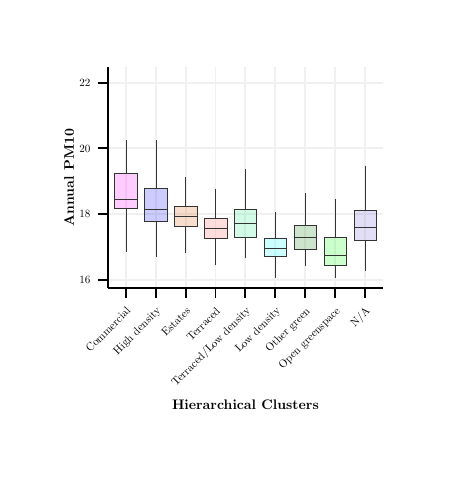
\begin{tikzpicture}[x=1pt,y=1pt]
\definecolor{fillColor}{RGB}{255,255,255}
\path[use as bounding box,fill=fillColor,fill opacity=0.00] (0,0) rectangle (142.64,152.15);
\begin{scope}
\path[clip] (  0.00,  0.00) rectangle (142.64,152.15);
\definecolor{fillColor}{RGB}{255,255,255}

\path[fill=fillColor] (  0.00,  0.00) rectangle (142.64,152.15);
\end{scope}
\begin{scope}
\path[clip] ( 28.95, 58.04) rectangle (128.41,137.92);
\definecolor{fillColor}{RGB}{255,255,255}

\path[fill=fillColor] ( 28.95, 58.04) rectangle (128.41,137.92);
\definecolor{drawColor}{gray}{0.94}

\path[draw=drawColor,line width= 0.7pt,line join=round] ( 28.95, 61.05) --
	(128.41, 61.05);

\path[draw=drawColor,line width= 0.7pt,line join=round] ( 28.95, 84.80) --
	(128.41, 84.80);

\path[draw=drawColor,line width= 0.7pt,line join=round] ( 28.95,108.55) --
	(128.41,108.55);

\path[draw=drawColor,line width= 0.7pt,line join=round] ( 28.95,132.30) --
	(128.41,132.30);

\path[draw=drawColor,line width= 0.7pt,line join=round] ( 35.43, 58.04) --
	( 35.43,137.92);

\path[draw=drawColor,line width= 0.7pt,line join=round] ( 46.25, 58.04) --
	( 46.25,137.92);

\path[draw=drawColor,line width= 0.7pt,line join=round] ( 57.06, 58.04) --
	( 57.06,137.92);

\path[draw=drawColor,line width= 0.7pt,line join=round] ( 67.87, 58.04) --
	( 67.87,137.92);

\path[draw=drawColor,line width= 0.7pt,line join=round] ( 78.68, 58.04) --
	( 78.68,137.92);

\path[draw=drawColor,line width= 0.7pt,line join=round] ( 89.49, 58.04) --
	( 89.49,137.92);

\path[draw=drawColor,line width= 0.7pt,line join=round] (100.30, 58.04) --
	(100.30,137.92);

\path[draw=drawColor,line width= 0.7pt,line join=round] (111.11, 58.04) --
	(111.11,137.92);

\path[draw=drawColor,line width= 0.7pt,line join=round] (121.93, 58.04) --
	(121.93,137.92);
\definecolor{drawColor}{gray}{0.20}

\path[draw=drawColor,line width= 0.1pt,line join=round] ( 46.25, 94.18) -- ( 46.25,111.73);

\path[draw=drawColor,line width= 0.1pt,line join=round] ( 46.25, 82.30) -- ( 46.25, 69.20);
\definecolor{fillColor}{RGB}{0,0,255}

\path[draw=drawColor,line width= 0.1pt,fill=fillColor,fill opacity=0.20] ( 42.19, 94.18) --
	( 42.19, 82.30) --
	( 50.30, 82.30) --
	( 50.30, 94.18) --
	( 42.19, 94.18) --
	cycle;

\path[draw=drawColor,line width= 0.1pt] ( 42.19, 86.72) -- ( 50.30, 86.72);

\path[draw=drawColor,line width= 0.1pt,line join=round] ( 35.43, 99.56) -- ( 35.43,111.42);

\path[draw=drawColor,line width= 0.1pt,line join=round] ( 35.43, 86.87) -- ( 35.43, 71.25);
\definecolor{fillColor}{RGB}{255,0,255}

\path[draw=drawColor,line width= 0.1pt,fill=fillColor,fill opacity=0.20] ( 31.38, 99.56) --
	( 31.38, 86.87) --
	( 39.49, 86.87) --
	( 39.49, 99.56) --
	( 31.38, 99.56) --
	cycle;

\path[draw=drawColor,line width= 0.1pt] ( 31.38, 90.35) -- ( 39.49, 90.35);

\path[draw=drawColor,line width= 0.1pt,line join=round] ( 89.49, 76.13) -- ( 89.49, 85.71);

\path[draw=drawColor,line width= 0.1pt,line join=round] ( 89.49, 69.70) -- ( 89.49, 61.67);
\definecolor{fillColor}{RGB}{0,255,255}

\path[draw=drawColor,line width= 0.1pt,fill=fillColor,fill opacity=0.20] ( 85.44, 76.13) --
	( 85.44, 69.70) --
	( 93.55, 69.70) --
	( 93.55, 76.13) --
	( 85.44, 76.13) --
	cycle;

\path[draw=drawColor,line width= 0.1pt] ( 85.44, 72.65) -- ( 93.55, 72.65);

\path[draw=drawColor,line width= 0.1pt,line join=round] (100.30, 80.80) -- (100.30, 92.39);

\path[draw=drawColor,line width= 0.1pt,line join=round] (100.30, 72.10) -- (100.30, 66.17);
\definecolor{fillColor}{RGB}{0,128,0}

\path[draw=drawColor,line width= 0.1pt,fill=fillColor,fill opacity=0.20] ( 96.25, 80.80) --
	( 96.25, 72.10) --
	(104.36, 72.10) --
	(104.36, 80.80) --
	( 96.25, 80.80) --
	cycle;

\path[draw=drawColor,line width= 0.1pt] ( 96.25, 76.32) -- (104.36, 76.32);

\path[draw=drawColor,line width= 0.1pt,line join=round] ( 67.87, 83.19) -- ( 67.87, 93.80);

\path[draw=drawColor,line width= 0.1pt,line join=round] ( 67.87, 76.10) -- ( 67.87, 66.22);
\definecolor{fillColor}{RGB}{255,85,85}

\path[draw=drawColor,line width= 0.1pt,fill=fillColor,fill opacity=0.20] ( 63.81, 83.19) --
	( 63.81, 76.10) --
	( 71.92, 76.10) --
	( 71.92, 83.19) --
	( 63.81, 83.19) --
	cycle;

\path[draw=drawColor,line width= 0.1pt] ( 63.81, 79.55) -- ( 71.92, 79.55);

\path[draw=drawColor,line width= 0.1pt,line join=round] ( 78.68, 86.53) -- ( 78.68,101.05);

\path[draw=drawColor,line width= 0.1pt,line join=round] ( 78.68, 76.44) -- ( 78.68, 68.97);
\definecolor{fillColor}{RGB}{37,229,137}

\path[draw=drawColor,line width= 0.1pt,fill=fillColor,fill opacity=0.20] ( 74.63, 86.53) --
	( 74.63, 76.44) --
	( 82.73, 76.44) --
	( 82.73, 86.53) --
	( 74.63, 86.53) --
	cycle;

\path[draw=drawColor,line width= 0.1pt] ( 74.63, 81.46) -- ( 82.73, 81.46);

\path[draw=drawColor,line width= 0.1pt,line join=round] (111.11, 76.32) -- (111.11, 90.32);

\path[draw=drawColor,line width= 0.1pt,line join=round] (111.11, 66.31) -- (111.11, 61.83);
\definecolor{fillColor}{RGB}{0,255,0}

\path[draw=drawColor,line width= 0.1pt,fill=fillColor,fill opacity=0.20] (107.06, 76.32) --
	(107.06, 66.31) --
	(115.17, 66.31) --
	(115.17, 76.32) --
	(107.06, 76.32) --
	cycle;

\path[draw=drawColor,line width= 0.1pt] (107.06, 69.91) -- (115.17, 69.91);

\path[draw=drawColor,line width= 0.1pt,line join=round] ( 57.06, 87.75) -- ( 57.06, 98.23);

\path[draw=drawColor,line width= 0.1pt,line join=round] ( 57.06, 80.30) -- ( 57.06, 70.60);
\definecolor{fillColor}{RGB}{212,85,0}

\path[draw=drawColor,line width= 0.1pt,fill=fillColor,fill opacity=0.20] ( 53.00, 87.75) --
	( 53.00, 80.30) --
	( 61.11, 80.30) --
	( 61.11, 87.75) --
	( 53.00, 87.75) --
	cycle;

\path[draw=drawColor,line width= 0.1pt] ( 53.00, 83.98) -- ( 61.11, 83.98);

\path[draw=drawColor,line width= 0.1pt,line join=round] (121.93, 86.13) -- (121.93,102.33);

\path[draw=drawColor,line width= 0.1pt,line join=round] (121.93, 75.20) -- (121.93, 64.15);
\definecolor{fillColor}{RGB}{106,90,205}

\path[draw=drawColor,line width= 0.1pt,fill=fillColor,fill opacity=0.20] (117.87, 86.13) --
	(117.87, 75.20) --
	(125.98, 75.20) --
	(125.98, 86.13) --
	(117.87, 86.13) --
	cycle;

\path[draw=drawColor,line width= 0.1pt] (117.87, 80.23) -- (125.98, 80.23);

\path[] ( 28.95, 58.04) rectangle (128.41,137.92);
\end{scope}
\begin{scope}
\path[clip] (  0.00,  0.00) rectangle (142.64,152.15);
\definecolor{drawColor}{RGB}{0,0,0}

\path[draw=drawColor,line width= 0.7pt,line join=round] ( 28.95, 58.04) --
	( 28.95,137.92);
\end{scope}
\begin{scope}
\path[clip] (  0.00,  0.00) rectangle (142.64,152.15);
\definecolor{drawColor}{RGB}{0,0,0}

\node[text=drawColor,anchor=base east,inner sep=0pt, outer sep=0pt, scale=  0.40] at ( 22.65, 59.67) {16};

\node[text=drawColor,anchor=base east,inner sep=0pt, outer sep=0pt, scale=  0.40] at ( 22.65, 83.42) {18};

\node[text=drawColor,anchor=base east,inner sep=0pt, outer sep=0pt, scale=  0.40] at ( 22.65,107.17) {20};

\node[text=drawColor,anchor=base east,inner sep=0pt, outer sep=0pt, scale=  0.40] at ( 22.65,130.92) {22};
\end{scope}
\begin{scope}
\path[clip] (  0.00,  0.00) rectangle (142.64,152.15);
\definecolor{drawColor}{RGB}{0,0,0}

\path[draw=drawColor,line width= 0.7pt,line join=round] ( 25.45, 61.05) --
	( 28.95, 61.05);

\path[draw=drawColor,line width= 0.7pt,line join=round] ( 25.45, 84.80) --
	( 28.95, 84.80);

\path[draw=drawColor,line width= 0.7pt,line join=round] ( 25.45,108.55) --
	( 28.95,108.55);

\path[draw=drawColor,line width= 0.7pt,line join=round] ( 25.45,132.30) --
	( 28.95,132.30);
\end{scope}
\begin{scope}
\path[clip] (  0.00,  0.00) rectangle (142.64,152.15);
\definecolor{drawColor}{RGB}{0,0,0}

\path[draw=drawColor,line width= 0.7pt,line join=round] ( 28.95, 58.04) --
	(128.41, 58.04);
\end{scope}
\begin{scope}
\path[clip] (  0.00,  0.00) rectangle (142.64,152.15);
\definecolor{drawColor}{RGB}{0,0,0}

\path[draw=drawColor,line width= 0.7pt,line join=round] ( 35.43, 54.54) --
	( 35.43, 58.04);

\path[draw=drawColor,line width= 0.7pt,line join=round] ( 46.25, 54.54) --
	( 46.25, 58.04);

\path[draw=drawColor,line width= 0.7pt,line join=round] ( 57.06, 54.54) --
	( 57.06, 58.04);

\path[draw=drawColor,line width= 0.7pt,line join=round] ( 67.87, 54.54) --
	( 67.87, 58.04);

\path[draw=drawColor,line width= 0.7pt,line join=round] ( 78.68, 54.54) --
	( 78.68, 58.04);

\path[draw=drawColor,line width= 0.7pt,line join=round] ( 89.49, 54.54) --
	( 89.49, 58.04);

\path[draw=drawColor,line width= 0.7pt,line join=round] (100.30, 54.54) --
	(100.30, 58.04);

\path[draw=drawColor,line width= 0.7pt,line join=round] (111.11, 54.54) --
	(111.11, 58.04);

\path[draw=drawColor,line width= 0.7pt,line join=round] (121.93, 54.54) --
	(121.93, 58.04);
\end{scope}
\begin{scope}
\path[clip] (  0.00,  0.00) rectangle (142.64,152.15);
\definecolor{drawColor}{RGB}{0,0,0}

\node[text=drawColor,rotate= 45.00,anchor=base east,inner sep=0pt, outer sep=0pt, scale=  0.40] at ( 37.36, 49.51) {Commercial};

\node[text=drawColor,rotate= 45.00,anchor=base east,inner sep=0pt, outer sep=0pt, scale=  0.40] at ( 48.17, 49.51) {High density};

\node[text=drawColor,rotate= 45.00,anchor=base east,inner sep=0pt, outer sep=0pt, scale=  0.40] at ( 58.99, 49.51) {Estates};

\node[text=drawColor,rotate= 45.00,anchor=base east,inner sep=0pt, outer sep=0pt, scale=  0.40] at ( 69.80, 49.51) {Terraced};

\node[text=drawColor,rotate= 45.00,anchor=base east,inner sep=0pt, outer sep=0pt, scale=  0.40] at ( 80.61, 49.51) {Terraced/Low density};

\node[text=drawColor,rotate= 45.00,anchor=base east,inner sep=0pt, outer sep=0pt, scale=  0.40] at ( 91.42, 49.51) {Low density};

\node[text=drawColor,rotate= 45.00,anchor=base east,inner sep=0pt, outer sep=0pt, scale=  0.40] at (102.23, 49.51) {Other green};

\node[text=drawColor,rotate= 45.00,anchor=base east,inner sep=0pt, outer sep=0pt, scale=  0.40] at (113.04, 49.51) {Open greenspace};

\node[text=drawColor,rotate= 45.00,anchor=base east,inner sep=0pt, outer sep=0pt, scale=  0.40] at (123.85, 49.51) {N/A};
\end{scope}
\begin{scope}
\path[clip] (  0.00,  0.00) rectangle (142.64,152.15);
\definecolor{drawColor}{RGB}{0,0,0}

\node[text=drawColor,anchor=base,inner sep=0pt, outer sep=0pt, scale=  0.50] at ( 78.68, 14.03) {\bfseries Hierarchical Clusters};
\end{scope}
\begin{scope}
\path[clip] (  0.00,  0.00) rectangle (142.64,152.15);
\definecolor{drawColor}{RGB}{0,0,0}

\node[text=drawColor,rotate= 90.00,anchor=base,inner sep=0pt, outer sep=0pt, scale=  0.50] at ( 16.70, 97.98) {\bfseries Annual PM10};
\end{scope}
\end{tikzpicture}
